\documentclass[a4paper,12pt]{article}

\RequirePackage{epsfig}

\setlength\hoffset{-0.5in}      %% these work quite well with a 12pt font
\setlength\voffset{-0.5in}
\setlength{\textwidth}{6.30in}
\setlength{\textheight}{9.0in}

\usepackage{graphicx}
\graphicspath{ {./img/} }

\bibliographystyle{unsrt}
\begin{document}

\begin{center}
{\Large\bf{Decentralised Blockchain Security Architecture for IoT and MQTT Brokers}} \\
      \vspace{5.0mm}
{\Large\bf{Project Plan}} \\
      \vspace{8mm}
      {\large\bf{Konrad Dryja}}  \\
      \vspace{5.0mm}
       {\tt k.dryja.15@abdn.ac.uk} \\
      \vspace{5.0mm}
      {\em Department of Computing Science,\\
       University of Aberdeen, Aberdeen AB24 3UE, UK} 
\end{center}


\section*{Introduction}

IoT is a growing field with presence getting larger from day to day. Equipment such as bus timetables, doorbells, thermostats or even pacemakers capable of sending alerts directly to emergency services is omnipresent. Sensitive data is very often handled (especially in the last example) and leak or misrepresentation can have catastrophic consequences. Additionally, those devices have limited computation power, which is sacrificed in favour of extended lifespan to avoid frequent maintenance and/or battery replacement. This makes it a very lucrative target for malicious actors. Researchers from University of Michigan performed a demo attack on a pacemaker, extracting personal information and changing the configuration.\cite{4531149} This example and more clearly presents a need for solution capable of securing and closing off access to unwanted agents.

What is more, those devices frequently do not directly communicate on a peer-to-peer basis, but instead pass through intermediary resource handling the distribution of data. MQTT Brokers\footnote{https://mqtt.org/} are one of them, providing a Publisher/Subscriber architecture, allowing for information exchange without the constant need of interconnectivity between clients, instead of relying on created topics used as a relay. MQTT is also not a piece of software, but rather just a standard describing the operation of such backend and leaves the implementation up to businesses. The documentation also clearly states that the security is not part of the standard, but rather leaves this decision up to the implementors. And while the transport of data can be assumed to remain secure (as MQTT operates over TCP/IP, thus encrypting the data using TLS), the access is often not. For example, an attack could be conducted, where malicious device communicates with the broker, impersonating another IoT hardware and finally 

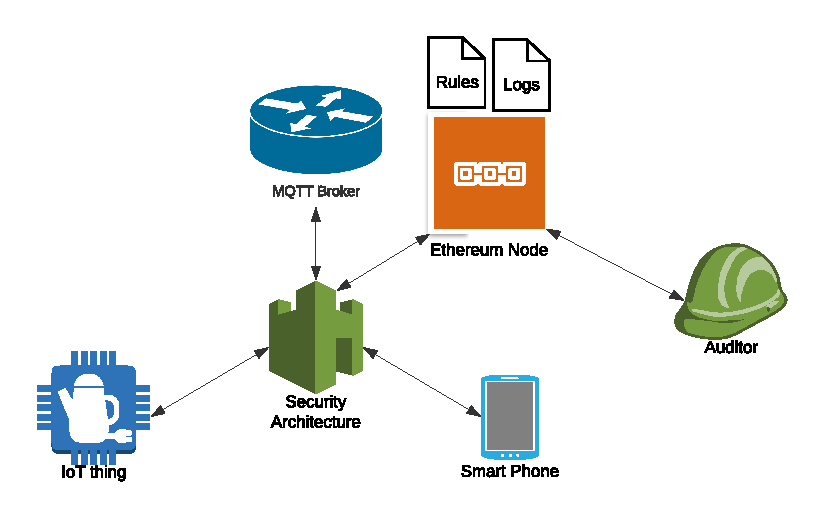
\includegraphics{iot_attack}

\section*{Goals}

This section should describe the the main goals of your project.
In other words, describe {\em what} it is that you want to do.
Are you building a tool or an application? What functionality 
already exists, and what will you have to do yourself?

Try to make it clear which goals are central to your project, and which
might be optional extras. Try to be realistic about making your
goals {\em achievable.}


\section*{Methodology}

This section should describe {\em how} you will conduct
your project. You should explain in general terms
the activities you will be carrying out during your project, such as:
%
\begin{itemize}
\item reading about related work -- either to get ideas on how to
      proceed, or to compare your approach with what was done before;
\item learing a new programming language or API;
\item learning about relevant technologies;
\item developing prototypes to test ideas;
\item testing and debugging early design choices.
\end{itemize}
%
The above examples are purely suggestions. You should try to think
of what would be appropriate for your specific project.

\section*{Resources Required}

You should mention here the hardware and software resources you will
require. Even if it seems obvious that you might only need Java and a PC, 
you should still say so!


\section*{Risk Assessment}

Try to describe possible circumstances (e.g. a particular piece of
technology doesn't work or is too expensive) that might cause
the project to become become infeasible. What would you have to do
or change to recover your project?

\section*{Timetable}

This section should describe the {\em schedule} for your project. 
You should describe the various activities you expect to perform
and their durations, along with any deadlines and deliverables.
It is often useful to collect all of this information in a
{\em Gantt chart}, as shown in Figure~\ref{fig:plan} below:

\begin{figure}[htb]
\begin{center}
% \includegraphics[scale=0.65]{ProjectPlan.eps}
\caption{Main Project Activities\label{fig:plan}}
\end{center}
\end{figure}

% For information, this figure was created using xfig, and 
% converted to encapsulated postscript by a command in the Makefile
% before being included as a graphic in the \LaTeX document.

Don't forget to add time at the end of your project for 
evaluation and writing-up! This could easily require 2-3 weeks.


\bibliography{ProjectPlan}

\end{document}
